%! TEX root = main.tex

In this section, we are interested in the scalability of PINNs.
In the weak scaling tests, we scaled $(2, 32, 8192)$ and $(3, 128, 8192)$ with 1, 2, 4, and 8 GPUs. 
As for the strong scaling tests, we scaled $(2, 32, 65536)$ and $(3, 128, 65536)$ with 1, 2, 4, and 8 GPUs. 
We will use an expression of $(N_l, N_n, N_{bs})\times N_{gpu}$ to denote how many GPUs are used and how many training points per batch on each GPU.
On the other, an expression of $(N_l, N_n, N_{bs}\times N_{gpu})$ denotes a case running on only one GPU but has $N_{bs}\times N_{gpu}$ training points per batch.

Figures \ref{fig:nl2-nn32-npts8192-weak-scaling} and \ref{fig:nl3-nn128-npts8192-weak-scaling} show the results of weak scaling tests.
These figures show the losses and errors of $u$ versus iterations on the left $y$-axis.
And for the other $y$-axis, we have the run times in hours versus iterations.

\begin{figure}[hbt!]
    \centering%
    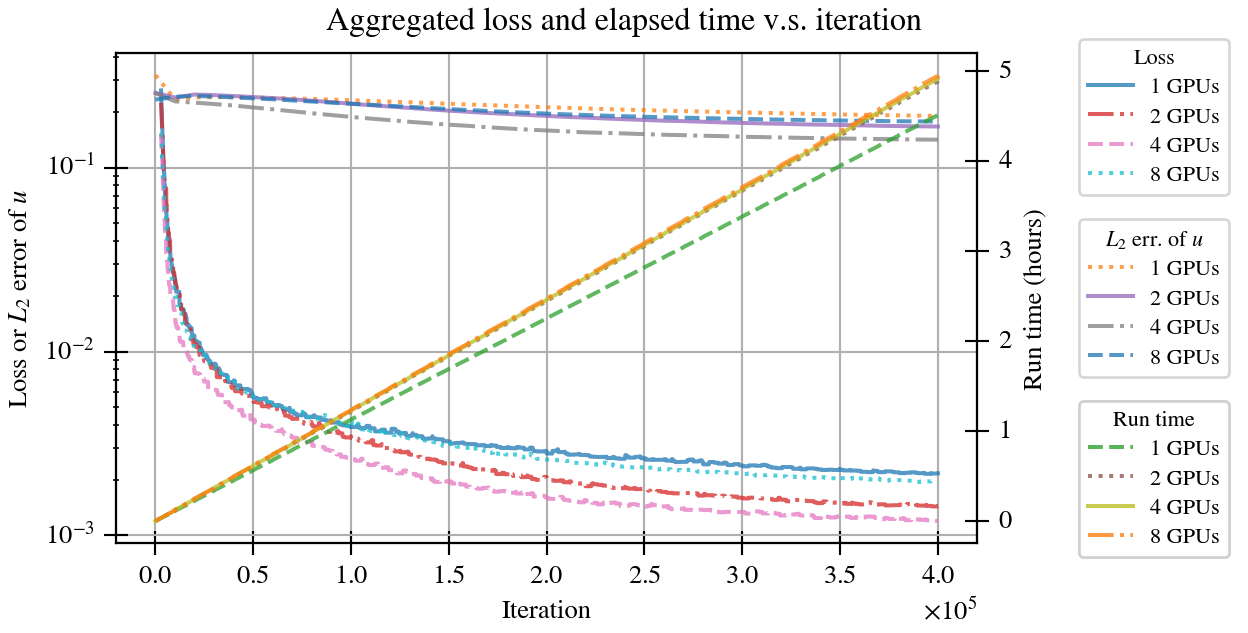
\includegraphics[width=0.9\linewidth]{tgv-2d-re100/scaling-tests/nl2-nn32-npts8192-weak-scaling.png}
    \caption[%
        Weak scaling: aggregated loss and run time v.s. iteration ($(N_l, N_n, N_{bs})$ $=$ $(2, 32, 8192)$)%
    ]{%
        Weak scaling: aggregated loss and run time v.s. iteration ($(N_l, N_n, N_{bs})$ $=$ $(2, 32, 8192)$)%
    }\label{fig:nl2-nn32-npts8192-weak-scaling}
\end{figure}

\begin{figure}[hbt!]
    \centering%
    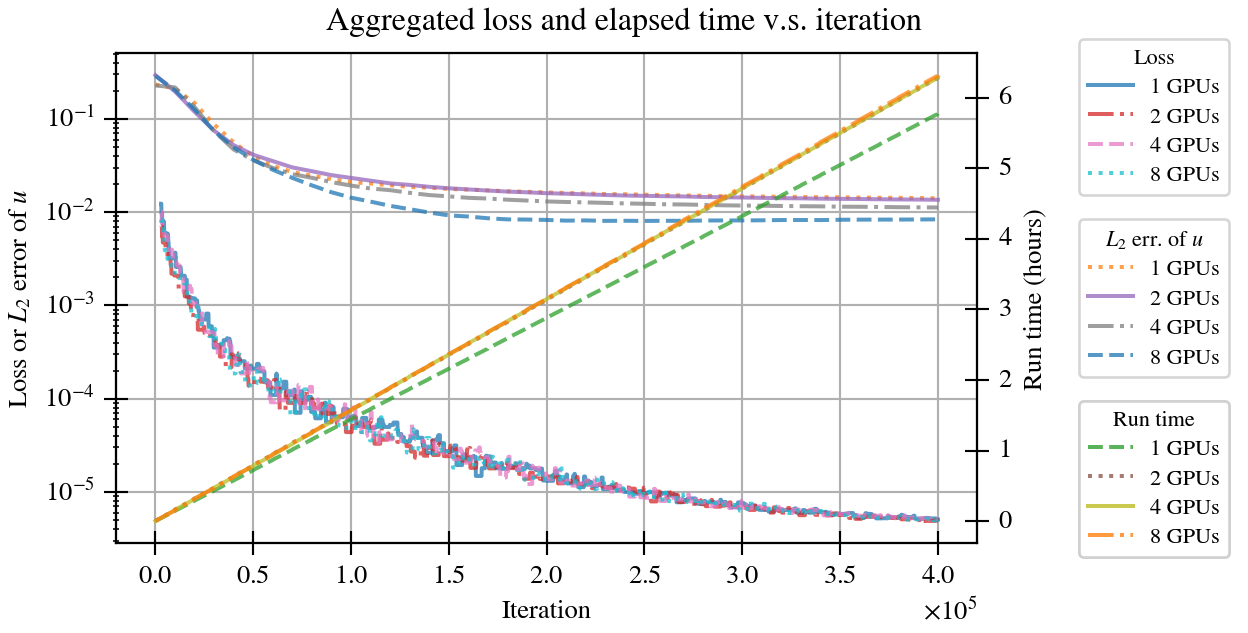
\includegraphics[width=0.9\linewidth]{tgv-2d-re100/scaling-tests/nl3-nn128-npts8192-weak-scaling.png}
    \caption[%
        Weak scaling: aggregated loss and run time v.s. iteration ($(N_l, N_n, N_{bs})$ $=$ $(3, 128, 8192)$)%
    ]{%
        Weak scaling: aggregated loss and run time v.s. iteration ($(N_l, N_n, N_{bs})$ $=$ $(3, 128, 8192)$)%
    }\label{fig:nl3-nn128-npts8192-weak-scaling}
\end{figure}

In weak scaling, because each GPU has the same amount of work loading, the run time versus iterations should be the same for different cases.
From figure \ref{fig:nl2-nn32-npts8192-weak-scaling} and \ref{fig:nl3-nn128-npts8192-weak-scaling}, we found that, except for the 1-GPU cases, cases with other GPUs match each other.
The reason that 1-GPU cases show different results may be that it does not have the latency overhead due to exchanging with other GPUs.

We further checked the losses and error histories and considered no significant difference between using different numbers of GPUs.
Note that while lines do not overlap on the figures, quantitatively speaking, the difference in the orders of magnitude is minor, as we will see in table \ref{table:weak-scaling-perf}. 

Theoretically, $(N_l, N_n, N_{bs})\times N_{gpu}$ is expected to equal to $(N_l, N_n, N_{bs}\times N_{gpu})$ in terms of losses and errors.
So the difference between using a different number of GPUs should be similar to the effect of using a different number of training points per batch on one GPU.
We will examine the effect of different $N_{bs}$ in section \ref{sec:pinn-2d-tgv-model-complexity}.
Instead, here we would like to check if it is true that $(N_l, N_n, N_{bs})\times N_{gpu}$ is equivalent to $(N_l, N_n, N_{bs}\times N_{gpu})$.
Figure \ref{fig:nl2-nn32-npts8192-multi-singl-gpus} shows the comparisons between $(2, 32, 8192)\times N_{gpu}$ and $(2, 32, 8192\times N_{gpu})$.
And figure \ref{fig:nl3-nn128-npts8192-multi-singl-gpus} shows the same comparisons between $(3, 128, 8192)\times N_{gpu}$ and $(3, 128, 8192\times N_{gpu})$.

\begin{figure}[hbt!]
    \centering%
    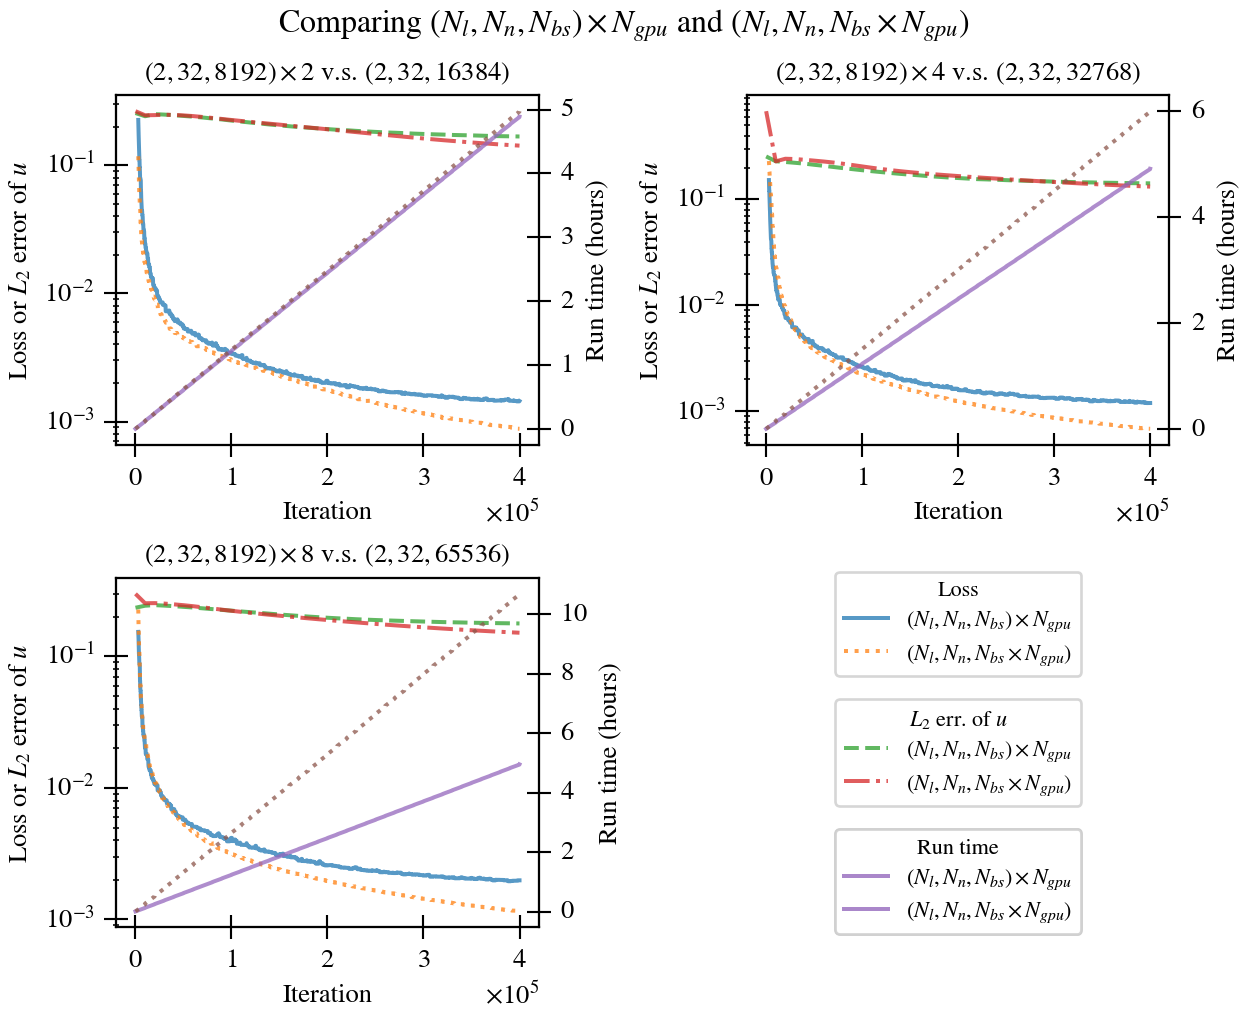
\includegraphics[width=0.9\linewidth]{tgv-2d-re100/scaling-tests/nl2-nn32-npts8192-multi-singl-gpus.png}
    \caption[%
        Comparing multi-GPU and single-GPU cases ($(N_l, N_n)$ $=$ $(2, 32)$)%
    ]{%
        Comparing multi-GPU and single-GPU cases ($(N_l, N_n)$ $=$ $(2, 32)$)%
    }\label{fig:nl2-nn32-npts8192-multi-singl-gpus}
\end{figure}

\begin{figure}[hbt!]
    \centering%
    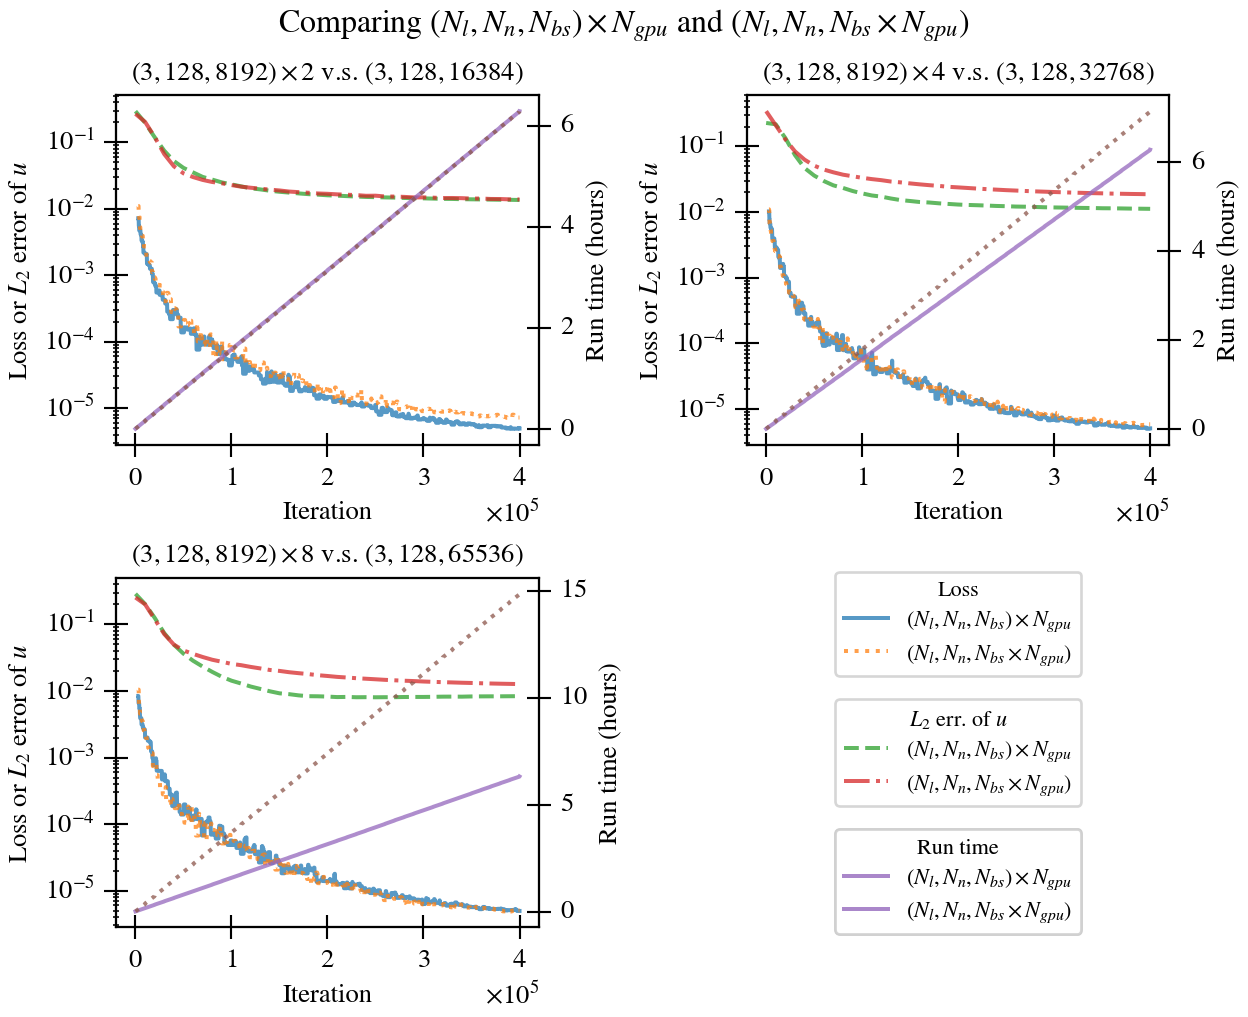
\includegraphics[width=0.9\linewidth]{tgv-2d-re100/scaling-tests/nl3-nn128-npts8192-multi-singl-gpus.png}
    \caption[%
        Comparing multi-GPU and single-GPU cases ($(N_l, N_n)$ $=$ $(3, 128)$)%
    ]{%
        Comparing multi-GPU and single-GPU cases ($(N_l, N_n)$ $=$ $(3, 128)$)%
    }\label{fig:nl3-nn128-npts8192-multi-singl-gpus}
\end{figure}

In these figures, it is expected that the run times are different and that the losses and errors are similar.
However, though losses and errors show similar trends between $(N_l, N_n, N_{bs})\times N_{gpu}$ and $(N_l, N_n, N_{bs}\times N_{gpu})$, visible differences exist.
In $(N_l, N_n)=(2, 32)$, losses stop improving earlier for multi-GPU cases, and multi-GPU cases have slightly worse errors.
On the other hand, for $(N_l, N_n)=(3, 128)$, the multi-GPU cases in general have better errors, though the loss histories do not show a noticeable difference.
The reason is unknown to us at this point.
The observation shows that $(N_l, N_n, N_{bs})\times N_{gpu}$ and $(N_l, N_n, N_{bs}\times N_{gpu})$ are not necessarily the same.
Nevertheless, we believe the differences are quantitatively minor if we consider their orders of magnitude.

\begin{table}[hbt!]
\centering
\singlespacing
\caption[
    PINNs, 2D TGV, $Re=100$: weak scaling performance for $(N_l, N_n, N_{bs})=(2, 32, 8192)$ and $(3, 128, 8192)$
]{
    Weak scaling performance for $(N_l, N_n, N_{bs})$ $=$ $(2, 32, 8192)$ and $(3, 128, 8192)$.%
    Time costs denote the wall time required to finish 400k training iterations in hours.%
    Efficiency here stands for weak scaling efficiency in $\%$.%
    The aggregated losses are those at the last iteration.%
    The $L_{2, sp-t}$ errors were the overall spatial-temporal errors at the last training iteration.%
}
\label{table:weak-scaling-perf}
\begin{tabular}{lcccccccc}
\toprule
 & \multicolumn{4}{c}{(2, 32, 8192)} & \multicolumn{4}{c}{(3, 128, 8192)} \\
\cmidrule(rl){2-5} \cmidrule(rl){6-9}
\multicolumn{1}{r}{GPUs} & 1 & 2 & 4 & 8 & 1 & 2 & 4 & 8 \\
\midrule
Time cost &  4.51 &  4.89 &  4.92 &  4.95 &  5.77 &  6.28 &  6.29 &  6.32 \\
\addlinespace
Efficiency & 100 & 92 & 92 & 91 & 100 & 92 & 92 & 91 \\
\addlinespace
Loss & 2.2e-03 & 1.5e-03 & 1.2e-03 & 2.1e-03 & 6.7e-06 & 5.3e-06 & 5.5e-06 & 5.3e-06 \\
\addlinespace
$L_{2,sp-t}$, $u$ & 1.9e-01 & 1.5e-01 & 1.2e-01 & 1.7e-01 & 1.3e-02 & 1.3e-02 & 1.0e-02 & 8.9e-03 \\
\addlinespace
$L_{2,sp-t}$, $v$ & 1.9e-01 & 1.5e-01 & 1.3e-01 & 1.8e-01 & 1.1e-02 & 1.2e-02 & 1.1e-02 & 9.6e-03 \\
\bottomrule
\end{tabular}
\end{table}


The quantitative results are listed in table \ref{table:weak-scaling-perf}.
The weak-scaling efficiencies are all above $90\%$.
The losses and errors are close in terms of the orders of magnitude.
PINNs generally have good weak-scaling if we define the workload using $N_{bs}$.
During training, each GPU calculates the gradients $\nabla_{\Theta} r(\Theta)$ independently, and then each training iteration only needs one reduction operation to calculate the averaged gradients across all GPUs.
A good weak scaling is thus expected.

Lastly, we examined the strong scaling.
Figure \ref{fig:nl2-nn32-npts65536-strong-scaling} shows the strong scaling results of $(2, 32, 65535)\times 1$, $(2, 32, 32768)\times 2$, $(2, 32, 16384)\times 4$, and $(2, 32, 8192)\times 8$.
Figure \ref{fig:nl3-nn128-npts65536-strong-scaling} shows the similar strong scaling tests for $(N_l, N_n)=(3, 128)$.
Quantitative results are listed in table \ref{table:strong-scaling-perf}. 

\begin{figure}[hbt!]
    \centering%
    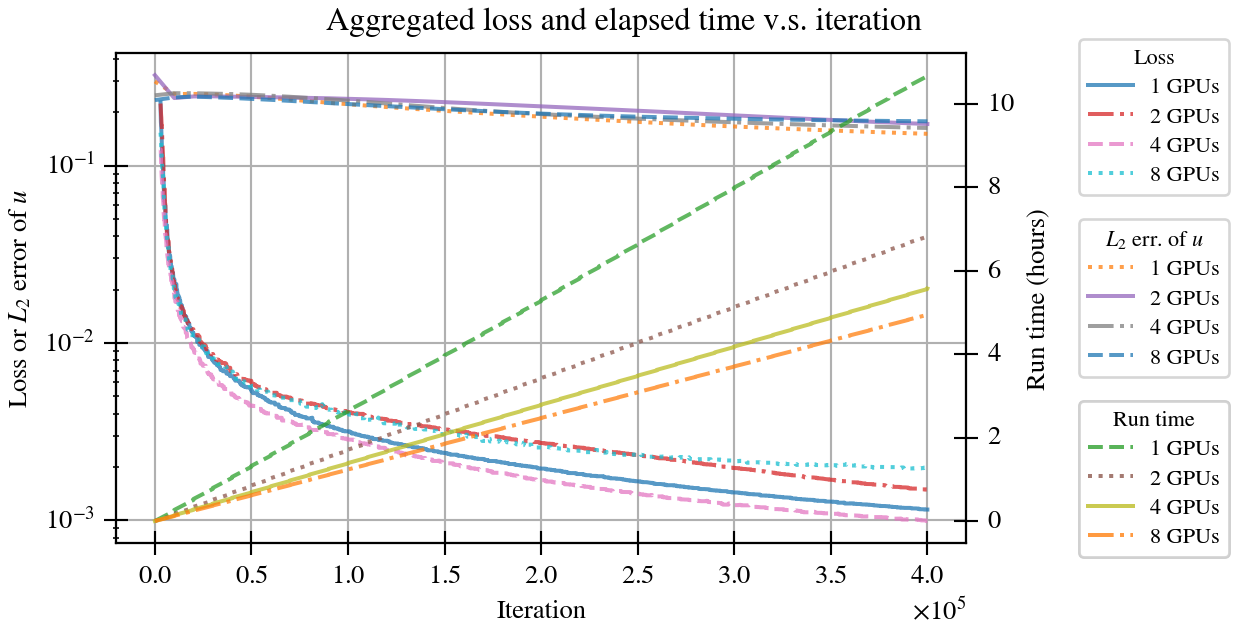
\includegraphics[width=0.9\linewidth]{tgv-2d-re100/scaling-tests/nl2-nn32-npts65536-strong-scaling.png}
    \caption[%
        Strong-scaling: aggregated loss and run time v.s. iteration ($(N_l, N_n, N_{bs})$ $=$ $(2, 32, 65535)$)%
    ]{%
        Strong-scaling: aggregated loss and run time v.s. iteration ($(N_l, N_n, N_{bs})$ $=$ $(2, 32, 65535)$)%
    }\label{fig:nl2-nn32-npts65536-strong-scaling}
\end{figure}

\begin{figure}[hbt!]
    \centering%
    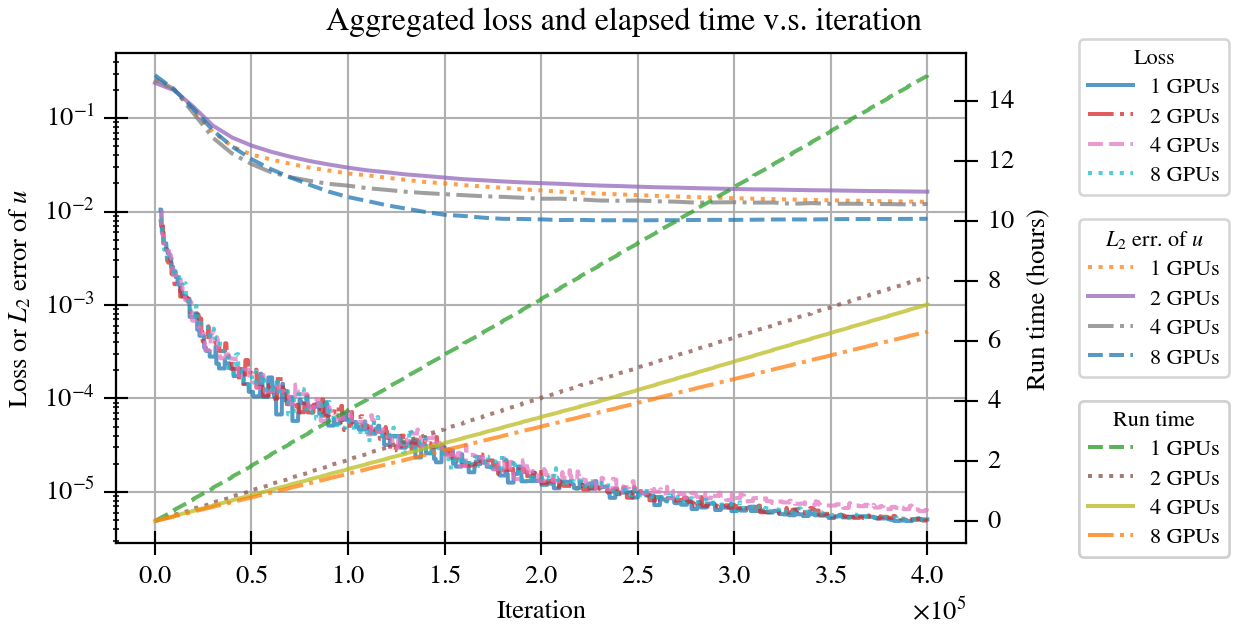
\includegraphics[width=0.9\linewidth]{tgv-2d-re100/scaling-tests/nl3-nn128-npts65536-strong-scaling.png}
    \caption[%
        Strong-scaling: aggregated loss and run time v.s. iteration ($(N_l, N_n, N_{bs})$ $=$ $(3, 128, 65535)$)%
    ]{%
        Strong-scaling: aggregated loss and run time v.s. iteration ($(N_l, N_n, N_{bs})$ $=$ $(3, 128, 65535)$)%
    }\label{fig:nl3-nn128-npts65536-strong-scaling}
\end{figure}

Theoretically, a good strong scaling result should show similar losses and errors.
Figures \ref{fig:nl2-nn32-npts65536-strong-scaling} and \ref{fig:nl3-nn128-npts65536-strong-scaling}, instead, exhibit some differences.
However, if we consider their orders of magnitude, we consider the differences minor.
This claim can be examined from table \ref{table:strong-scaling-perf}.
On the other hand, the results show deteriorating strong scaling efficiencies.
The worse strong scaling is caused by only dividing the training points across GPUs, while the model itself is not divided.  
The model complexity also contributes to the work loading.
We do not have a clear way to divide a model and distribute the work loading across GPUs.
Neither do we have means to exclude the model's contribution to the work loading and correctly calculate the strong scaling efficiencies and speedups.
Lacking these knowledges limited our investigation into the strong scaling of PINNs.

\begin{table}[hbt!]
\centering
\singlespacing
\caption[
    PINNs, 2D TGV, $Re=100$: strong scaling performance for $(N_l$, $N_n$, $N_{bs})$ $=$ $(2$, $32$, $65536)$ and $(3$, $128$, $65536)$
]{
    Strong scaling performance for $(N_l$, $N_n$, $N_{bs})$ $=$ $(2$, $32$, $65536)$ and $(3$, $128$, $65536)$.%
    Time costs denote the wall time required to finish 400k training iterations in hours.%
    Efficiency here stands for strong scaling efficiency in $\%$.%
    The aggregated losses were those at the last iteration.%
    The $L_{2,sp-t}$ errors were the overall spatial-temporal errors at the last training iteration.%
}
\label{table:strong-scaling-perf}
\begin{tabular}{lcccccccc}
\toprule
 & \multicolumn{4}{c}{(2, 32, 65536)} & \multicolumn{4}{c}{(3, 128, 65536)} \\
\cmidrule(rl){2-5} \cmidrule(rl){6-9}
\multicolumn{1}{r}{GPUs} & 1 & 2 & 4 & 8 & 1 & 2 & 4 & 8 \\
\midrule
Time cost & 10.69 &  6.82 &  5.57 &  4.95 & 14.79 &  8.12 &  7.23 &  6.32 \\
\addlinespace
Speedup & 1.0x & 1.6x & 1.9x & 2.2x & 1.0x & 1.8x & 2.0x & 2.3x \\
\addlinespace
Efficiency & 100 & 78 & 48 & 27 & 100 & 91 & 51 & 29 \\
\addlinespace
Loss & 1.2e-03 & 1.5e-03 & 1.0e-03 & 2.1e-03 & 5.1e-06 & 5.2e-06 & 6.7e-06 & 5.3e-06 \\
\addlinespace
$L_{2,sp-t}$, $u$ & 1.4e-01 & 1.6e-01 & 1.5e-01 & 1.7e-01 & 1.1e-02 & 1.6e-02 & 1.2e-02 & 8.9e-03 \\
\addlinespace
$L_{2,sp-t}$, $v$ & 1.4e-01 & 1.6e-01 & 1.5e-01 & 1.8e-01 & 1.0e-02 & 1.7e-02 & 1.2e-02 & 9.6e-03 \\
\bottomrule
\end{tabular}
\end{table}

% vim:ft=tex